\documentclass{VUMIFPSkursinis}
\usepackage{algorithmicx}
\usepackage{algorithm}
\usepackage{algpseudocode}
\usepackage{amsfonts}
\usepackage{amsmath}
\usepackage{bm}
\usepackage{caption}
\usepackage{color}
\usepackage{float}
\usepackage{graphicx}
\usepackage{listings}
\usepackage{subfig}
\usepackage{wrapfig}

% Titulinio aprašas
\university{Vilniaus universitetas}
\faculty{Matematikos ir informatikos fakultetas}
\department{Programų sistemų katedra}
\papertype{Kursinis darbas}
\title{Blokų grandinių duomenų bazės finansinių duomenų kaupimui}
\titleineng{Blockchain databases for financial data}
\status{3 kurso 3 grupės studentas}
\author{Matas Savickis}
% \secondauthor{Vardonis Pavardonis}   % Pridėti antrą autorių
\supervisor{Vytautas Valaitis, Asist., Dr.}
\date{Vilnius – \the\year}

% Nustatymai
% \setmainfont{Palemonas}   % Pakeisti teksto šriftą į Palemonas (turi būti įdiegtas sistemoje)
\bibliography{bibliografija}

\begin{document}
\maketitle

\tableofcontents

\sectionnonum{Įvadas}
Kiekvieno sėkmingo verslo pagrindas yra pinigai. Vystant betkokį verslą didėją bendradarbiavimas 
su kitomis įmonėmis ir finansinėmis įstaigomis. Iškyla poreikis sekti pinigines tranzakcijas ir įsipareigojimus 
su kitomis įmonėmis. Praeityje tokie duomys buvo saugomi realicinėse duomenų bazėse. Nors tokiu būdų saugomi
duomenys būna pasiekiami greitai, tačiau iškyla problema, kad tokių duomenų saugojimui yra paskiriama trečia 
šalis ir mums tenka ja pasitikėti, kad duomenys nebus pakeisti ar ištrinti. Šią problemą padeda išspręsti ,,Blockchain" 
technologija. Blockchain yra duomenų saugojimo būdas padedantis užtikrinti duomenų integralumą
panaikinant poreikį priklausyti nuo trečiosios šalies. Blockchain technologija buvo sukurta Satoshi Nakamoto 2008 metais.
Nakomoto blockchain dizainą implementavo sukurdamas kripto valiutą ,,Bitcoin" 2009 metais. Nors neiškarto buvo suprasta 
kripto valiutų vertė per pastarajį penkmetį pasaulis patyrė kriptovaliutų bumą. Blockchain technologija taip pat buvo pritaikyta
naujų duomenų bazių tokių kaip Hyperledger, Corda ir Bigchain kūrime. Šios duomenų bazės pasižymi pagrindiniais blockchain
technologijos bruožais: duomenų nekeičiamumu, kriptografiniu saugumu ir decentralizacija. Šiame darbe aš sieksiu ištirti ir palyginti
NoSQL duomenų bazes su blockchain duomenų bazėmis finansinių duomenų saugojime. Darbe bus lyginamas duomenų perdavimo greitis, 
duomenų bazių sunaudojami kompiuteriniai ištekliai ir bazių plėtimo galimybės. Darbu bus siekiama išskirti pagrindiniai blokinių grandinių 
ir NoSQL duomenų bažių privalumai ir trūkumai, bei pasiūlyti panaudojimo atvejus abiem duomenų bazių tipams.


\section{Medžiagos darbo tema dėstymo skyriai}

\subsection{Duomenų bazių greičiai}
\subsection{Duomenų bazių energijos sanaudos}
\subsection{Duomenų bazių plėtimo galimybės}


\sectionnonum{Rezultatai ir išvados}
Rezultatų ir išvadų dalyje turi būti aiškiai išdėstomi pagrindiniai darbo
rezultatai (kažkas išanalizuota, kažkas sukurta, kažkas įdiegta) ir pateikiamos
išvados (daromi nagrinėtų problemų sprendimo metodų palyginimai, teikiamos
rekomendacijos, akcentuojamos naujovės).

\printbibliography[heading=bibintoc]  % Šaltinių sąraše nurodoma panaudota
% literatūra, kitokie šaltiniai. Abėcėlės tvarka išdėstomi darbe panaudotų
% (cituotų, perfrazuotų ar bent paminėtų) mokslo leidinių, kitokių publikacijų
% bibliografiniai aprašai.  Šaltinių sąrašas spausdinamas iš naujo puslapio.
% Aprašai pateikiami netransliteruoti. Šaltinių sąraše negali būti tokių
% šaltinių, kurie nebuvo paminėti tekste.

% \sectionnonum{Sąvokų apibrėžimai}
\sectionnonum{Santrumpos}
Sąvokų apibrėžimai ir santrumpų sąrašas sudaromas tada, kai darbo tekste
vartojami specialūs paaiškinimo reikalaujantys terminai ir rečiau sutinkamos
santrumpos.

\appendix  % Priedai
% Prieduose gali būti pateikiama pagalbinė, ypač darbo autoriaus savarankiškai
% parengta, medžiaga. Savarankiški priedai gali būti pateikiami ir
% kompaktiniame diske. Priedai taip pat numeruojami ir vadinami. Darbo tekstas
% su priedais susiejamas nuorodomis.

\section{Niauroninio tinklo struktūra}
\begin{figure}[H]
    \centering
    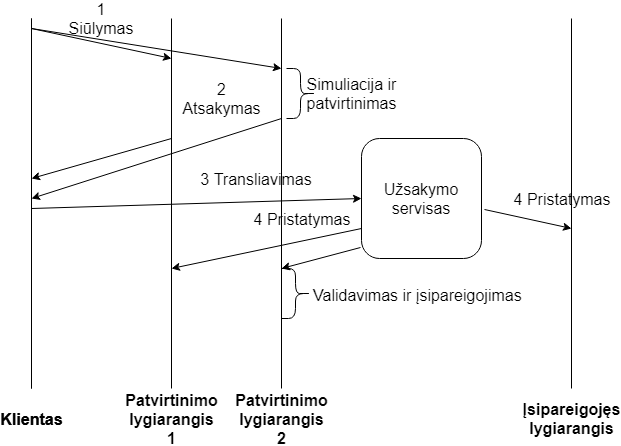
\includegraphics[scale=0.5]{img/MLP}
    \caption{Paveikslėlio pavyzdys}
    \label{img:mlp}
\end{figure}


\section{Eksperimentinio palyginimo rezultatai}
% tablesgenerator.com - converts calculators (e.g. excel) tables to LaTeX
\begin{table}[H]\footnotesize
  \centering
  \caption{Lentelės pavyzdys}
  {\begin{tabular}{|l|c|c|} \hline
    Algoritmas & $\bar{x}$ & $\sigma^{2}$ \\
    \hline
    Algoritmas A  & 1.6335    & 0.5584       \\
    Algoritmas B  & 1.7395    & 0.5647       \\
    \hline
  \end{tabular}}
  \label{tab:table example}
\end{table}

\end{document}
